\chapter{Implementation}

\section{Working-Methodology}

In the events of initiation of an audio session, the system will go through the\\
following steps in order to successfully start streaming:\\

 The first step of course involves pointing to the media the user wishes to play.\\
 This involves any kind of Audio / Video source from any of the compatible providers \\
 ex: Spotify, YouTube, Gaana, etc.\\
 
 Time to pass the Gems ! Next , choose the client to share the Content link to.\\
  This will send it to the STUN / TURN servers to successfully reach the target device\\

 The  middleware server helps in\\
 case of any NAT related issues and delivers the content to the correct device associated with you.\\

Finally the content reaches your intended device.\\
It parses, identifies and resolves the data, fetches the media content \\
from the corresponding service and proceeds to play it. Handling the audio buffer over to the Hi-Res DAC .\\

The Hi-Res DAC converts the binary audio buffer into a high precision analog sound signal.\\
 This signal is handed over to a Hi-Fi Class AB 15 watt Audio Amplifier.\\

Finally the Hi-Fi Class AB amplifier drives the 2.4 Inch speakers producing your awaited tune.\\


\begin{figure}[H]
  \caption{Design}
  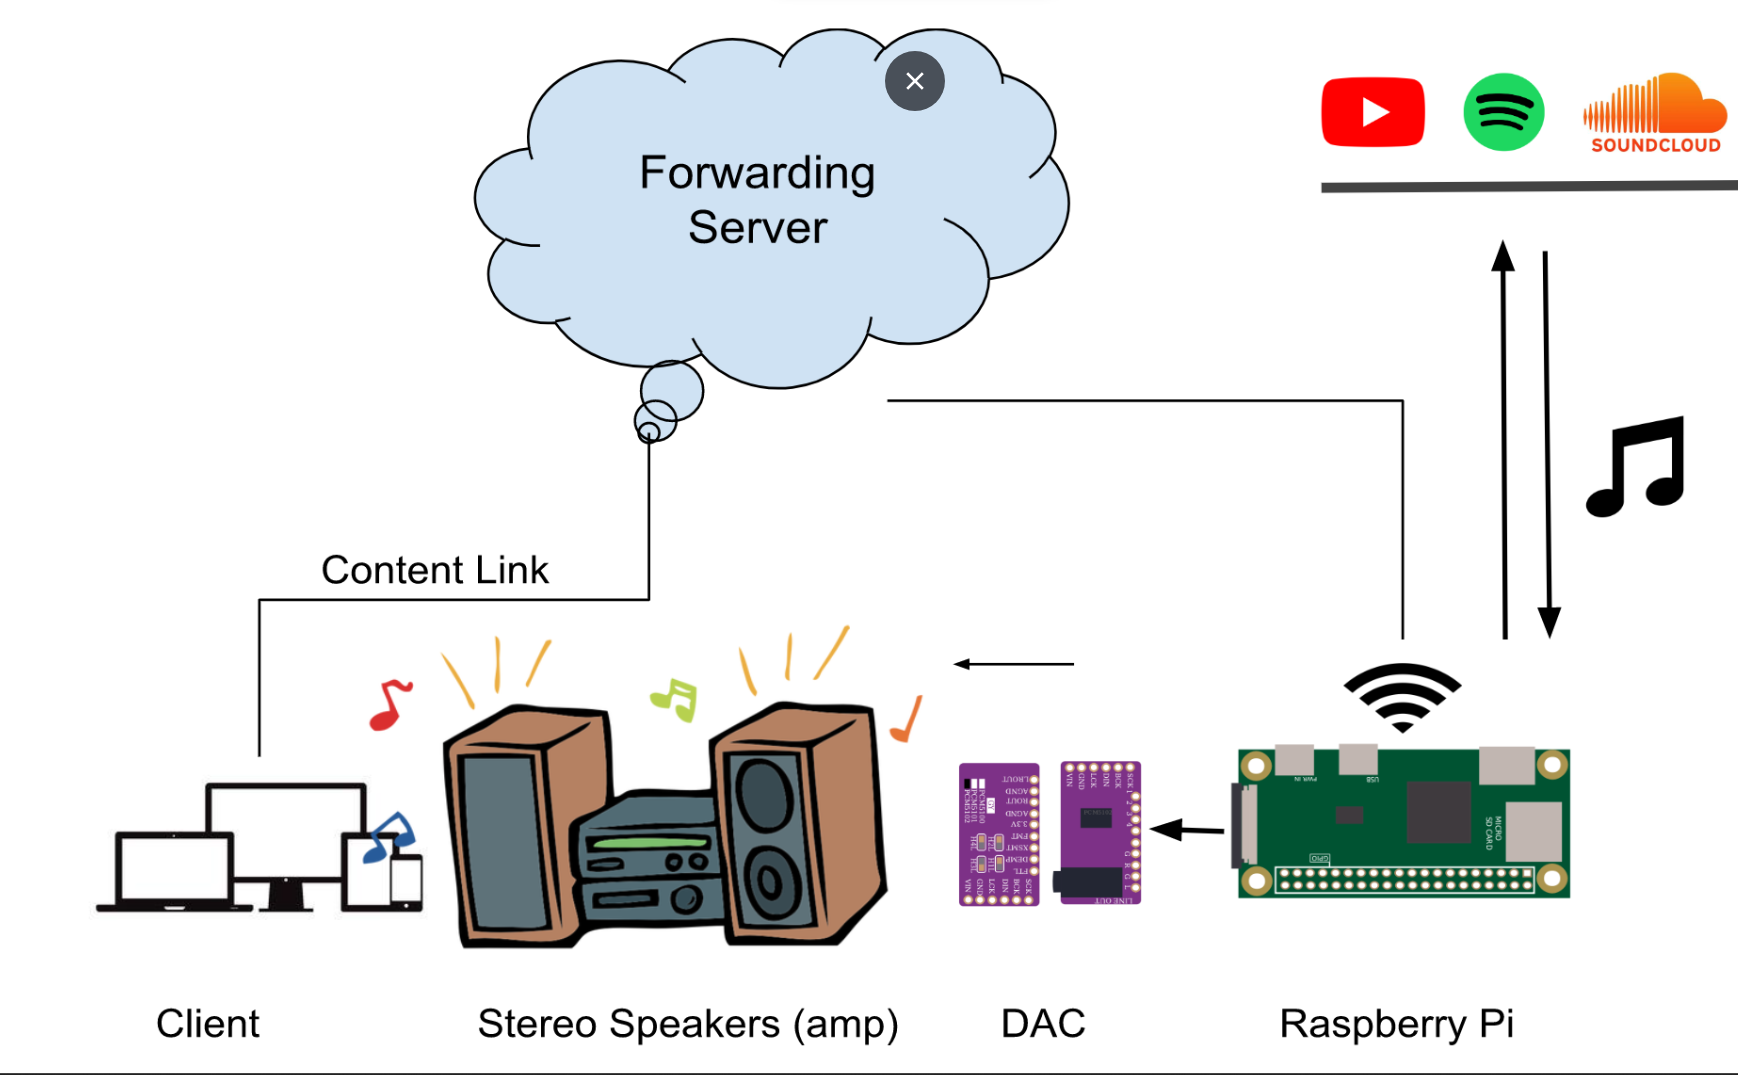
\includegraphics[scale=.4]{./implement.png}
  \\[0.2in]
\end{figure}
\begin{figure}[H]
  \caption{Home Page}
  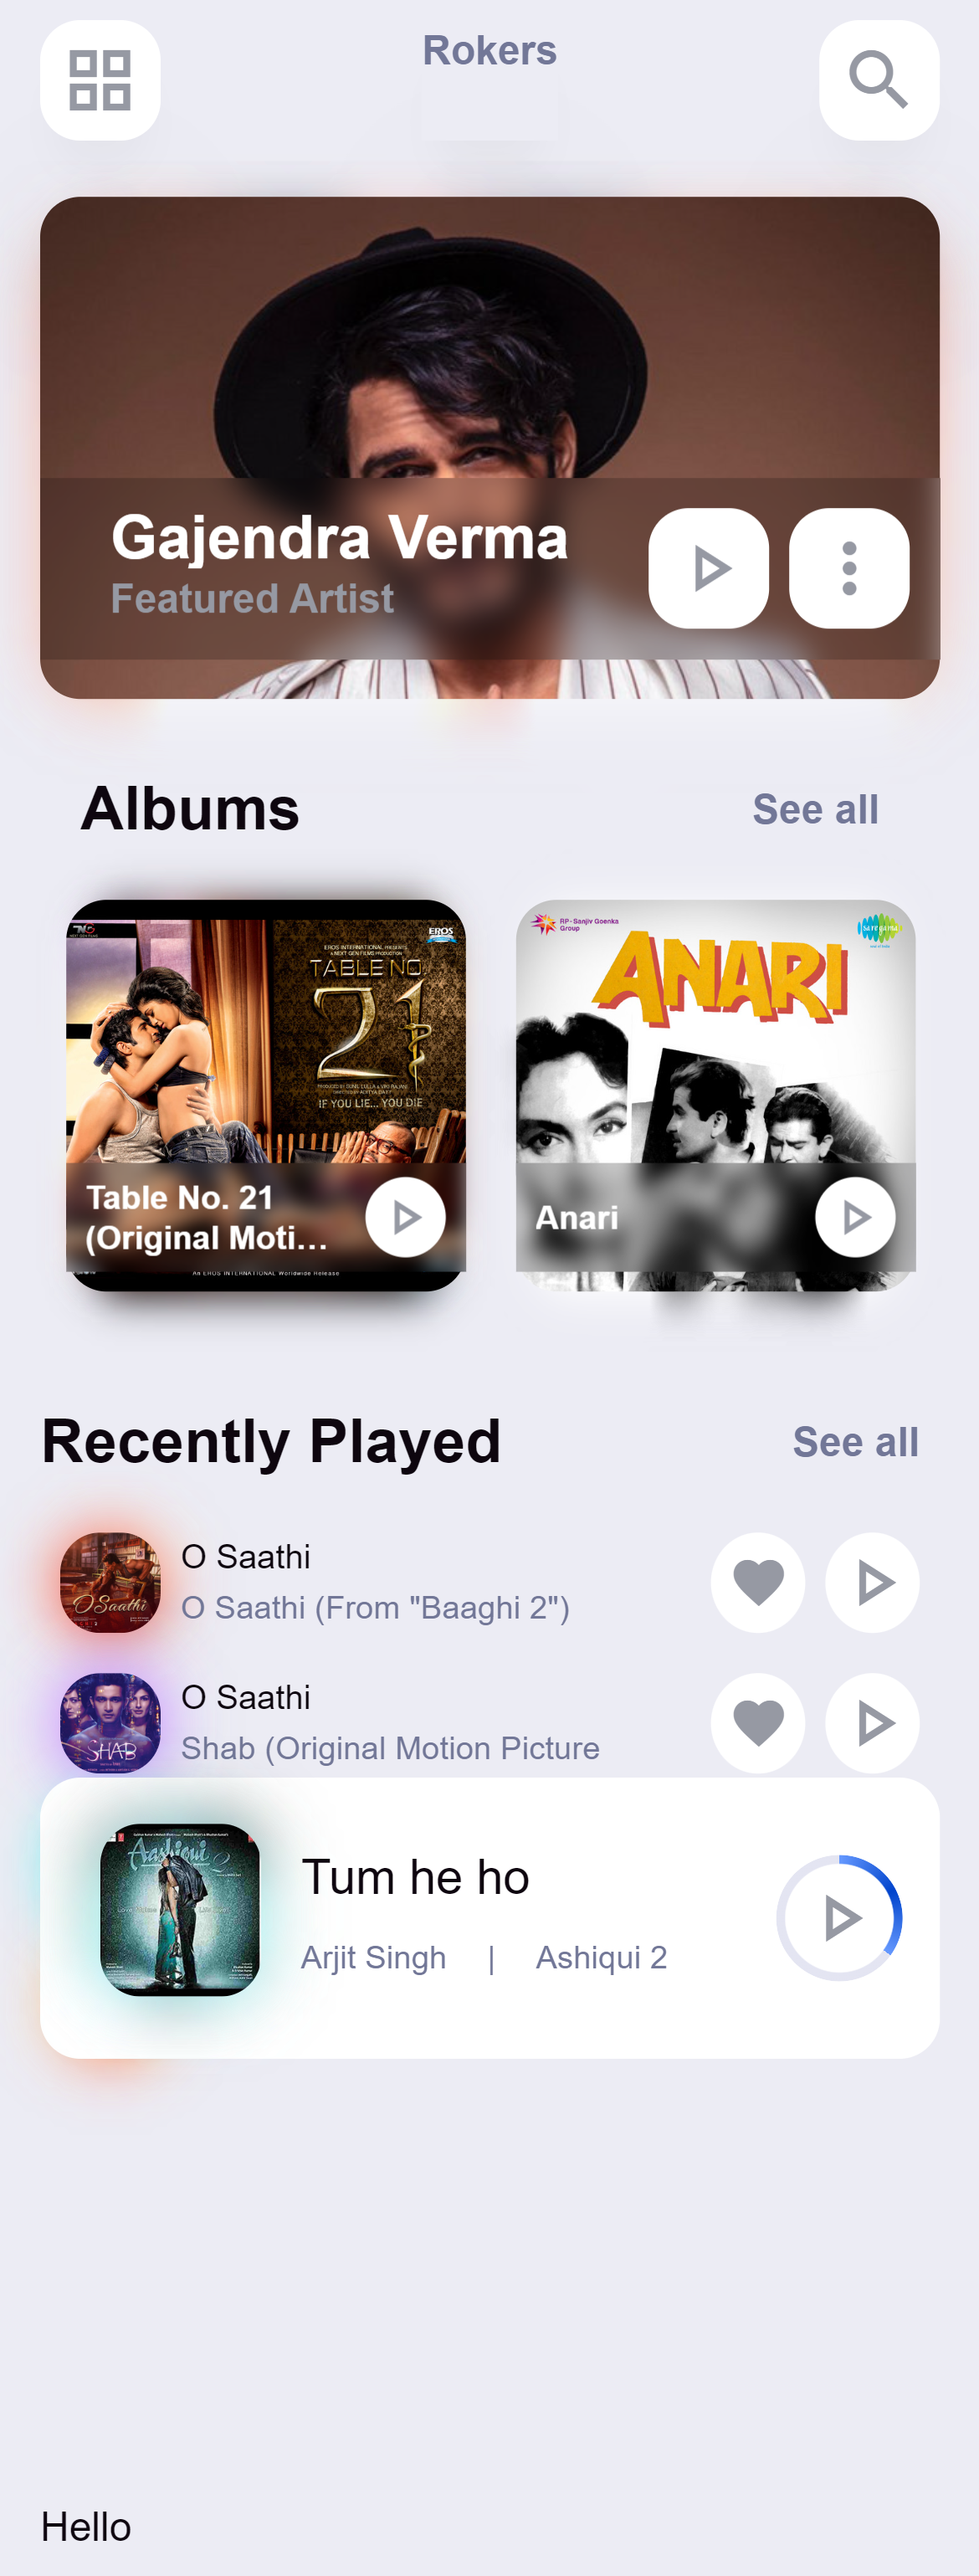
\includegraphics[scale=.2]{./screenshot.png}

\end{figure}
\begin{figure}[H]
  \caption{Albums View}
  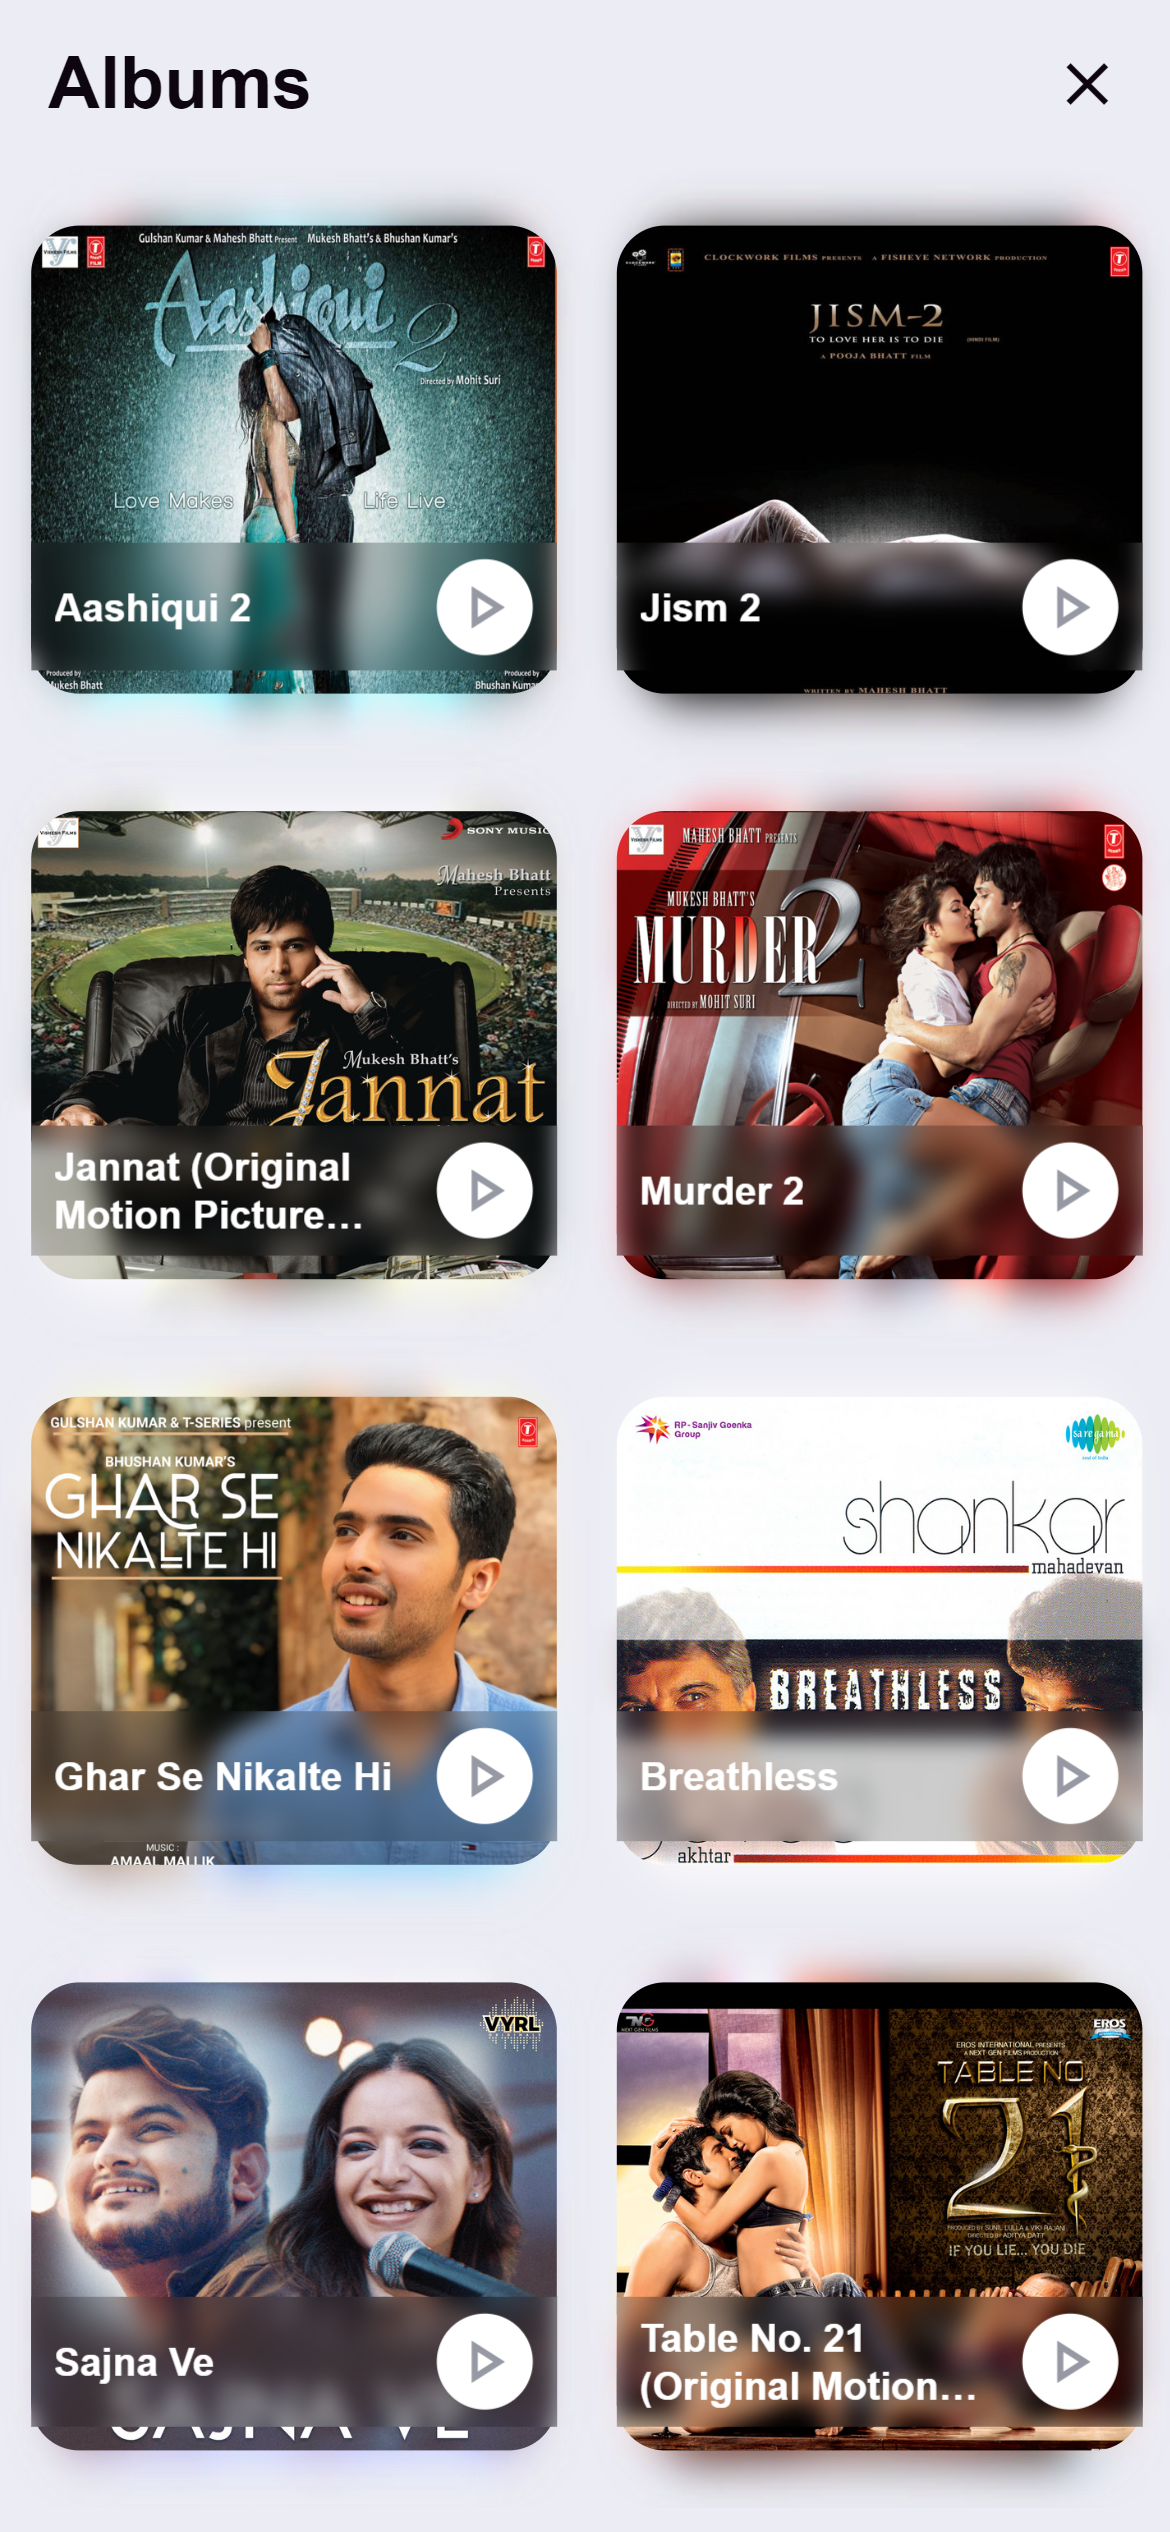
\includegraphics[scale=.2]{./screenshot1.png}

\end{figure}
\begin{figure}[H]
  \caption{Search View}
  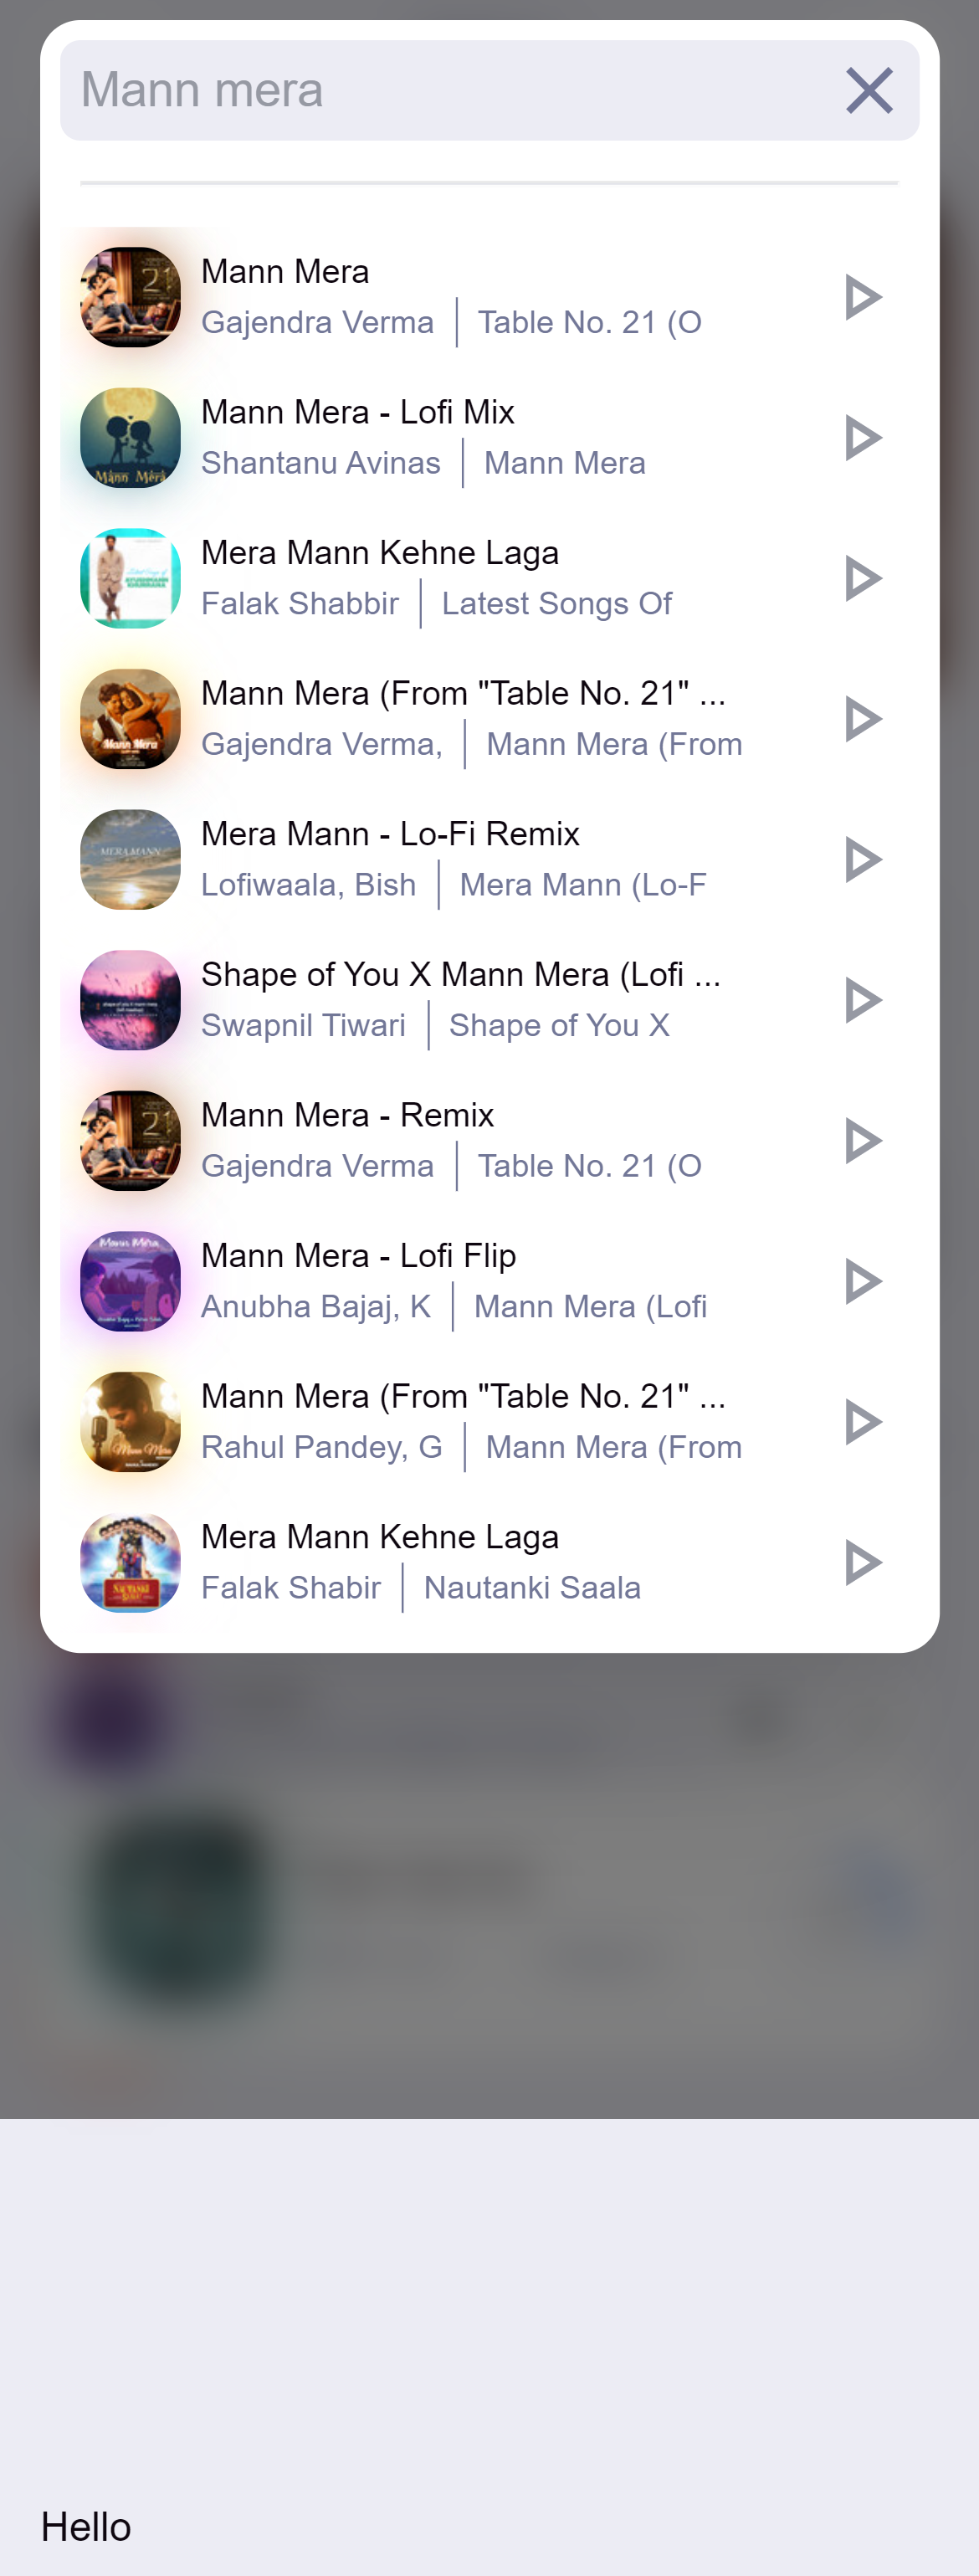
\includegraphics[scale=.2]{./screenshot2.png}

\end{figure}
\begin{figure}[H]
  \caption{Recents View}
  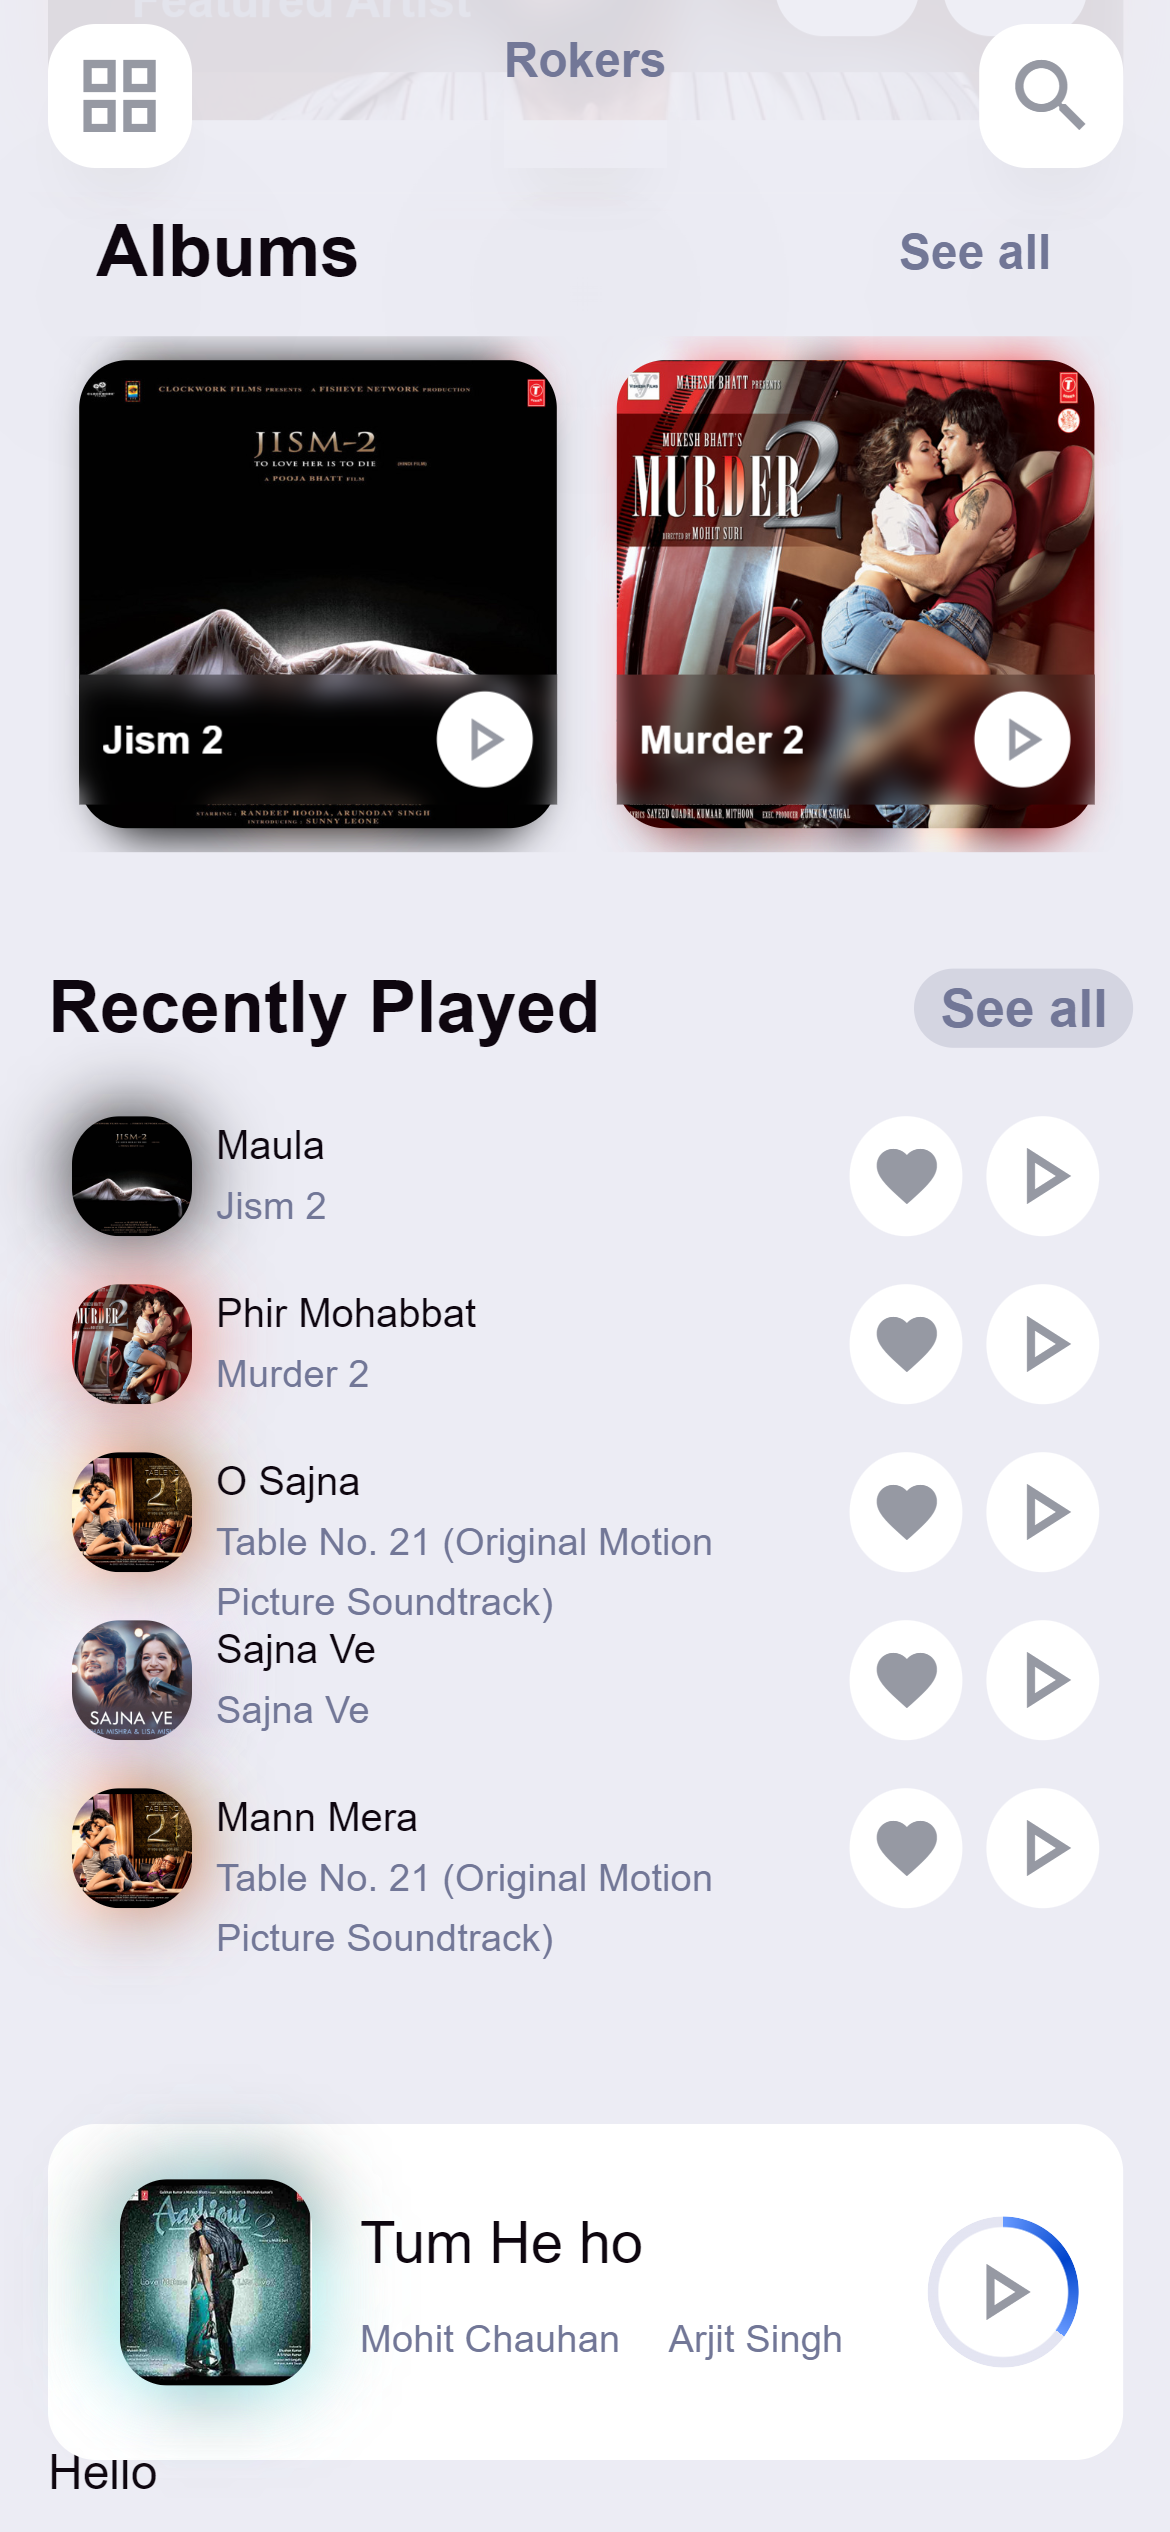
\includegraphics[scale=.2]{./screenshot3.png}

\end{figure}

\pagebreak

